\chapter{REFERENCIAL TEÓRICO}

\section{Manufatura Aditiva}
O princípio fundamental da manufatura aditiva (MA) consiste em fabricar um modelo tridimensional de forma integrada, dispensando a necessidade de planejar as operações de maneira individual. Este processo começa com um modelo tridimensional digital, frequentemente desenvolvido via Computer Aided Design (CAD), cujas especificações são interpretadas por um software fatiador. Este software ajusta parâmetros e gera instruções essenciais para a máquina de manufatura aditiva fabricar o modelo físico. Estas instruções, variando conforme a tecnologia e o modelo específico da impressora, são comumente transmitidas através do Gcode. O Gcode é uma linguagem de programação que direciona a impressora 3D sobre como construir o objeto, incluindo informações sobre movimentos, velocidades e temperaturas. Além do Gcode, informações adicionais como arquivos de imagens podem ser utilizadas para complementar o processo.

Uma das características principais da MA é a rapidez na qual é possível criar protótipos diretamente de modelos digitais, por conta disso, em um contexto de desenvolvimento de produto, o termo prototipagem rápida era utilizado. Entretanto, conforme a MA foi se aperfeiçoando era perceptível a capacidade dessas tecnologias não só se aterem à produção de protótipos, mas também de peças utilizadas em produtos finais. Além disso, o termo prototipagem rápida não considerava o princípio básico que unia essas tecnologias e assim o termo manufatura aditiva foi apresentado e adotado pela \textit{American Society for Testing and Materials} (ASTM) \cite{gibson15}.

Atualmente, existe uma grande variedade de tecnologias e processos de manufatura aditiva. Os métodos de impressão 3D variam na maneira como depositam o material, como extrusão, sinterização a  laser e estereolitografia. Eles também diferem nos princípios físicos que utilizam, como fusão, cura por luz e aglutinação. Além disso, os materiais que podem ser utilizados incluem plásticos, resinas, metais e cerâmicas. Como mencionado anteriormente, um dos métodos de manufatura aditiva mais populares é a tecnologia FDM, entretanto existem diversas outras tecnologias que tem crescido muito em popularidade como as tecnologias baseadas na cura seletiva de resinas, \textit{stereolithography} (SLA) e \textit{Masked stereolithography Apparatus} (MSLA), além de outras tecnologias menos acessíveis, mas com aplicações em diversas industrias, como por exemplo \textit{selective laser melting} (SLM) e \textit{Selective laser Sintering} (SLS) \cite{bikas16}. Na figura \ref{fig:MA_industrias} podemos observar a distribuição do uso de tecnologias MA por tipo de industria.   

\begin{figure}[H]
    \begin{center}
    \caption{Distribuição de uso de MA nas industrias}
    % 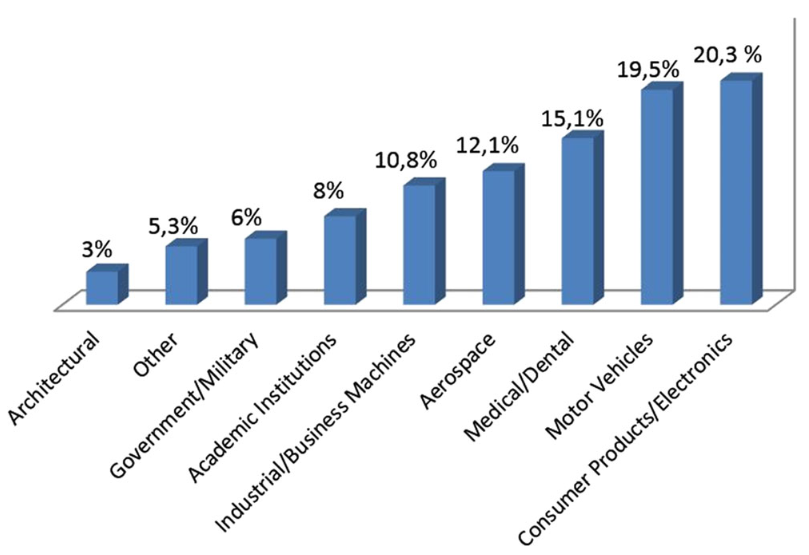
\includegraphics[scale=0.6]{bikas15industries}
    
    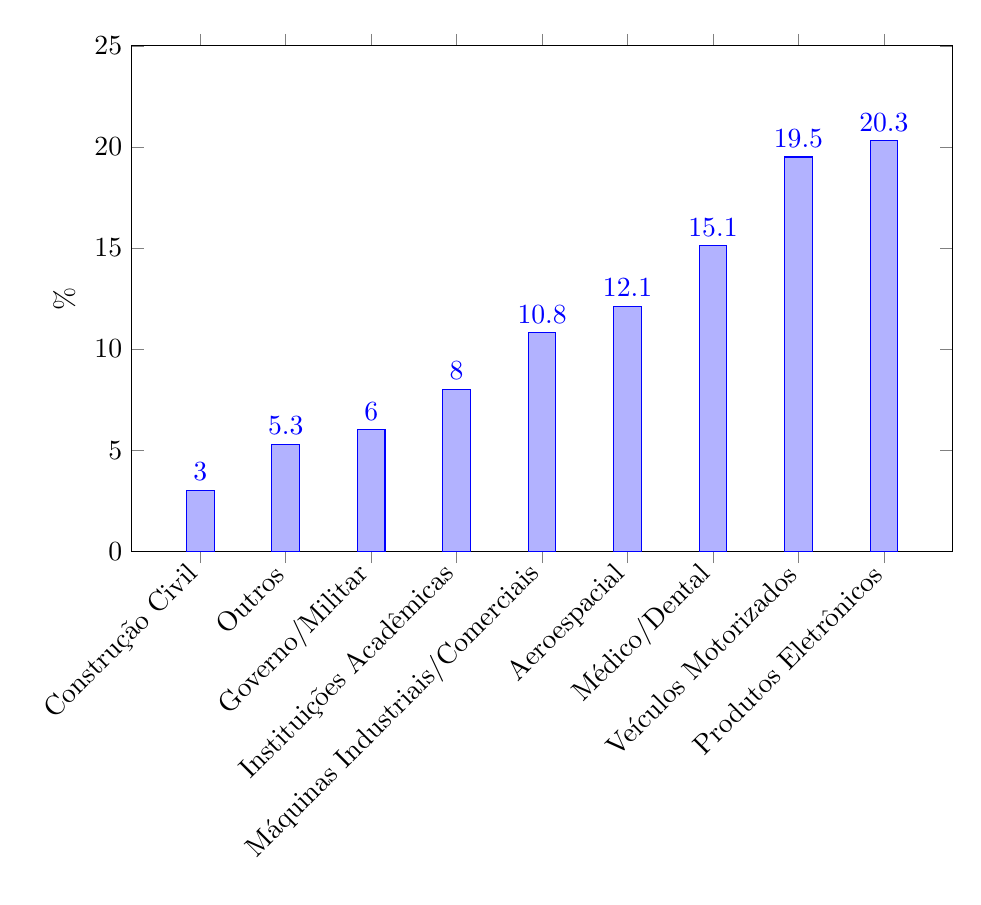
\begin{tikzpicture}
        \begin{axis}[
            ybar,
            width=12cm,
            height=8cm,
            enlarge x limits=0.1,
            ylabel={\%},
            symbolic x coords={
                Construção Civil, 
                Outros, 
                Governo/Militar, 
                Instituições Acadêmicas, 
                Máquinas Industriais/Comerciais, 
                Aeroespacial, 
                Médico/Dental, 
                Veículos Motorizados, 
                Produtos Eletrônicos
            },
            xtick=data,
            nodes near coords,
            nodes near coords align={vertical},
            x tick label style={rotate=45, anchor=east, align=center},
            ymin=0,
            ymax=25
        ]
        \addplot coordinates {
            (Construção Civil, 3)
            (Outros, 5.3)
            (Governo/Militar, 6)
            (Instituições Acadêmicas, 8)
            (Máquinas Industriais/Comerciais, 10.8)
            (Aeroespacial, 12.1)
            (Médico/Dental, 15.1)
            (Veículos Motorizados, 19.5)
            (Produtos Eletrônicos, 20.3)
        };
        \end{axis}
    \end{tikzpicture}

    {\footnotesize Fonte: Adaptado de \citeauthor{bikas16}, \citeyear{bikas16}}
    \label{fig:MA_industrias}
    \end{center}
\end{figure}

\section{\textit{Fused Deposition Modeling}}
\textit{Fused Deposition Modeling} (FDM) ou \textit{Fused Filament Fabrication} (FFF) é uma das tecnologias MA mais populares como mencionado anteriormente. Ela se consiste por depositar material através de um processo onde um filamento de material é forçado dentro de uma câmara através, geralmente, de rolos dentados onde em uma região específica esse material é liquefeito. Por conta da pressão criada pelo filamento adentrando a câmara dentro do extrusor, ainda no estado sólido, o material liquefeito é extrudado através de um bocal, comumente fabricado de bronze. Então, o filamento liquefeito é depositado em uma plataforma de forma a percorrer a trajetória desejada utilizando mecanismos movidos de forma controlada, geralmente por motores de passos. O processo é repetido camada por camada, de forma que elas estejam apoiadas por camadas anteriores e a primeira camada continue fixa na plataforma ou cama, até que o processo finalize \cite{turner14}. A Figura \ref{fig:fdm_ex} ilustra este processo.

\begin{figure}[H]
    \begin{center}
    \caption{Principio e processo de impressão para FDM}
    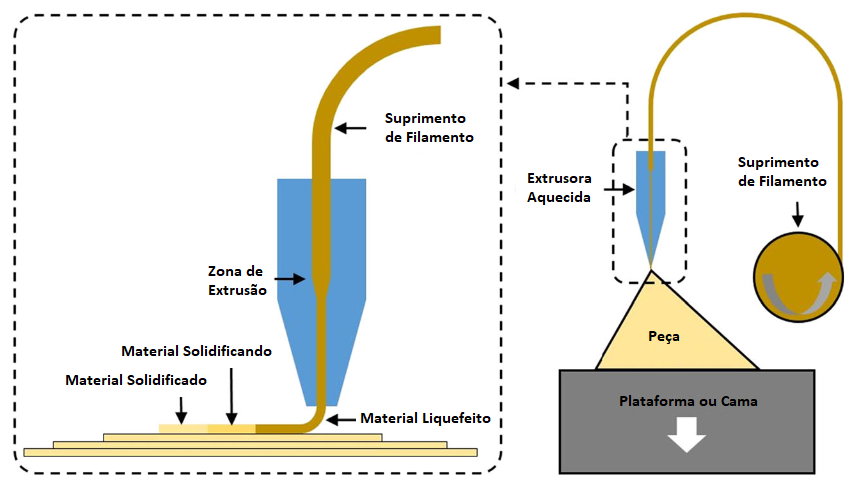
\includegraphics[scale=0.6]{bikas2015FDM}

    {\footnotesize Fonte:Adaptado de \citeauthor{bikas16}, \citeyear{bikas16}}
    \label{fig:fdm_ex}
    \end{center}
\end{figure}

Este procedimento meticuloso exige a colaboração de vários componentes essenciais da impressora 3D. Estes componentes incluem:

Extrusora: A extrusora é responsável por derreter o filamento de material termoplástico e extrudá-lo em forma de filamento derretido. Ela consiste em um bico aquecido (\textit{hotend}) que funde o material e um motor que empurra o filamento através do bico. Alguns modelos mais avançados podem ter extrusoras duplas para imprimir com materiais diferentes ou suportes solúveis.

Mesa de impressão: A mesa de impressão é a superfície onde o objeto está sendo construído. Ela é aquecida em muitas impressoras FDM para ajudar a aderência do material à superfície. Além disso, algumas mesas de impressão têm características especiais, como superfícies texturizadas ou magnéticas, para facilitar a aderência e a remoção do objeto após a conclusão.

Plataforma de construção: A plataforma de construção é o suporte físico onde a mesa de impressão é montada. Ela pode ser ajustada em altura para nivelar a superfície de impressão e garantir que a primeira camada do objeto seja depositada com precisão.

Motor de movimento: Impressoras 3D FDM possuem motores de movimento que controlam a posição da extrusora e da mesa de impressão ao longo dos eixos X, Y e Z. Geralmente são motores de passo e seus movimentos de rotação são geralmente convertidos em movimentos lineares através de correias ou parafusos de rosca trapezoidal.

Filamento: O filamento é o material de alimentação para a impressora 3D. Ele é um longo fio de plástico termoplástico que é inserido na extrusora e derretido durante o processo de impressão. Os filamentos vêm em várias cores e tipos de material, dependendo do objeto a ser impresso.

Sistema de controle: A eletrônica de controle inclui a placa-mãe da impressora, que recebe comandos do software, em geral no formato Gcode, e os traduz em movimentos dos motores, controle de temperatura da extrusora e da mesa de impressão, velocidade dos ventiladores entre outros acessórios. Ela também pode ter uma tela de exibição e controles para operação manual.

A Figura \ref{fig:impressora3d_comp} indica alguns destes componentes e a Figura \ref{fig:slicer_inter} mostra a interface de um fatiador.

\begin{figure}[H]
    \centering
    \caption{Indicação dos componentes de uma impressora 3D}
    \includegraphics[scale=0.04]{impressora3d_comp}
    \label{fig:impressora3d_comp}
\end{figure}

\begin{figure}[H]
    \centering
    \caption{Interface do fatiador PrusaSlicer}
    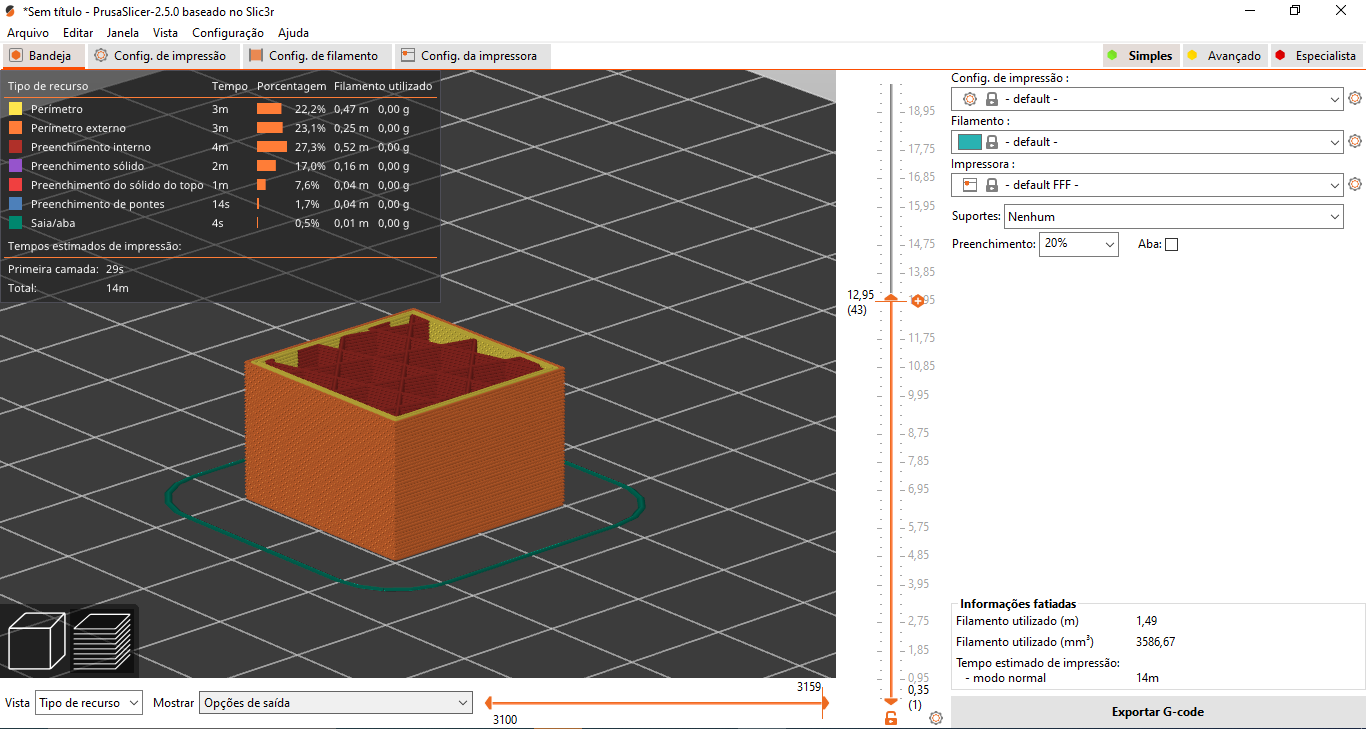
\includegraphics[scale=0.4]{slicer_inter}
    \label{fig:slicer_inter}
\end{figure}

Podemos separar, de maneira simplificada, o \textit{software} de impressoras 3D FDM em algumas etapas: fatiamento (\textit{slicing}) ou geração de comando, geração de trajetória e controle ou controle de trajetória. A etapa de geração de comando, realizado pelo fatiador, onde o volume do modelo é dividido em camadas, definindo um percurso através de uma sequência de comandos. Esses comandos controlam os movimentos a serem realizados, definição de configurações, o controle da temperatura e outros dispositivos. Já na etapa de geração de trajetória, os comandos criados pelo fatiador (\textit{slicer}) na etapa anterior são interpretadas, entretanto esses comandos não descrevem em detalhes. Portanto, é necessário a definição do comportamento que a impressora deve tomar para cumprir o comando interpretado, no caso de um comando de movimento por exemplo precisamos construir a trajetória dos eixos para poder realizar o comando com sucesso, assim chamamos esta etapa de geração de trajetória. Podemos, antes de prosseguir para a próxima etapa, utilizar de técnicas de controle para melhorar a performance da execução dos comandos, por exemplo utilizar os sensores de temperatura para modificar a taxa de aquecimento do bico extrusor, ou utilizar essas técnicas de controle para alterar a trajetória construída na etapa anterior de maneira a contribuir para a qualidade da impressão. Por fim, temos a etapa de geração de sinais, onde a impressora precisa converter as abstrações definidas sobre seus dispositivos em sinais que são responsáveis em controla-los. Por exemplo, converter as características do movimento de um eixo em uma série de pulsos elétricos que controlam os motores de passo. 

\subsection{Geração de Comando}

O Gcode (Código G) é uma linguagem de programação usada em impressoras 3D e máquinas CNC para controlar o movimento e as ações da máquina durante o processo de fabricação. Ele é muito utilizado pelos fatiadores para representar os comandos para a impressora 3D. O Gcode é composto por uma série de comandos textuais, cada um com um formato específico. Aqui estão alguns elementos-chave da estrutura típica de um comando G-code:

\begin{itemize}
    \item Prefixo (Código G): Todo comando G-code começa com a letra 'G', que indica que é um comando de movimento ou função.
    \item Número do Comando: Após o 'G', segue um número que identifica o tipo específico de comando. Por exemplo, 'G0' é frequentemente usado para mover rapidamente a cabeça de impressão para uma posição, enquanto 'G1' é usado para movimentos de impressão lineares.
    \item Parâmetros: Após o número do comando, podem seguir-se parâmetros adicionais. Esses parâmetros variam dependendo do comando, mas podem incluir coordenadas de posicionamento (X, Y, Z), velocidades de movimento, taxas de alimentação, temperaturas e outros valores relevantes.
    \item Comentários: O G-code também pode incluir comentários precedidos por um ponto e vírgula (;) ou entre parênteses (). Os comentários não afetam a execução do programa, mas ajudam a documentar o código para facilitar a compreensão.
    \item Fim de Linha: Cada comando G-code é normalmente concluído com um caractere de fim de linha, como o retorno de carro ('\textbackslash n') ou a combinação de retorno de carro e nova linha ('\textbackslash r \textbackslash n'), dependendo do sistema.
\end{itemize}

\begin{figure}[H]
    \centering
    \caption{Exemplo de um arquivo Gcode}
    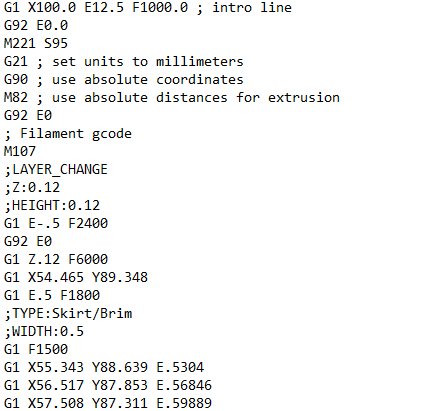
\includegraphics[scale=0.6]{Gcode_ex}
    \label{fig:gcode_ex}
\end{figure}

\subsection{Geração de trajetória}
A geração de trajetória é o processo que define o comportamento dos eixos da impressora ao longo do tempo com base nos comandos interpretados, incluindo além dos eixos de movimento, eixos de temperatura, potência dos ventiladores e de taxa de extrusão por exemplo. Esses diferentes componentes precisam coordenados e seu comportamento necessita de ser definido para que seja possível converter essas abstrações no mundo físico posteriormente. No caso dos eixos de movimento, uma estratégia para se construir esse comportamento são as curvas de velocidade trapezoidal \cite{yu20}. 

\subsection{Curvas de velocidade trapezoidal}
A construção das curvas de velocidade trapezoidal se da no objetivo de se deslocar de uma posição e velocidade inicial para uma posição e velocidade final, considerando uma velocidade máxima. Assim, se utiliza uma configuração de aceleração armazenada na impressora a fim de definir o comportamento das variações de velocidade. Vale lembrar que os comandos de movimento podem possuir atuação de múltiplos eixos e dado o objetivo das condições iniciais e finais de cada eixo se darem ao mesmo tempo, é utilizado o modulo do vetor de velocidade, composto pelas velocidades de cada eixo.

A partir dessas características, ao construir o perfil de velocidade em uma situação onde se tenha tempo suficiente para atingir a velocidade máxima, com base na aceleração definida pela impressora, o perfil de velocidade tem uma aparência trapezoidal (seções 1, 3 e 4), justificando o nome da estratégia. Entretanto, caso não seja possível alcançar a velocidade máxima dentro do tempo e deslocamento possível para o movimento, o perfil de velocidade passa a possuir uma aparência triangular (seção 2), causada pelo fato de não existir mais uma seção onde é mantida a velocidade máxima \cite{yu20,klipperkinematic}. A Figura \ref{fig:trap_triang} mostra um perfil de velocidade de uma sequência de quatro movimentos, apresentando seções trapezoidais e triangulares.

\begin{figure}[H]
    \centering
    \caption{Perfil de velocidade - Curva trapezoidal de velocidade}
    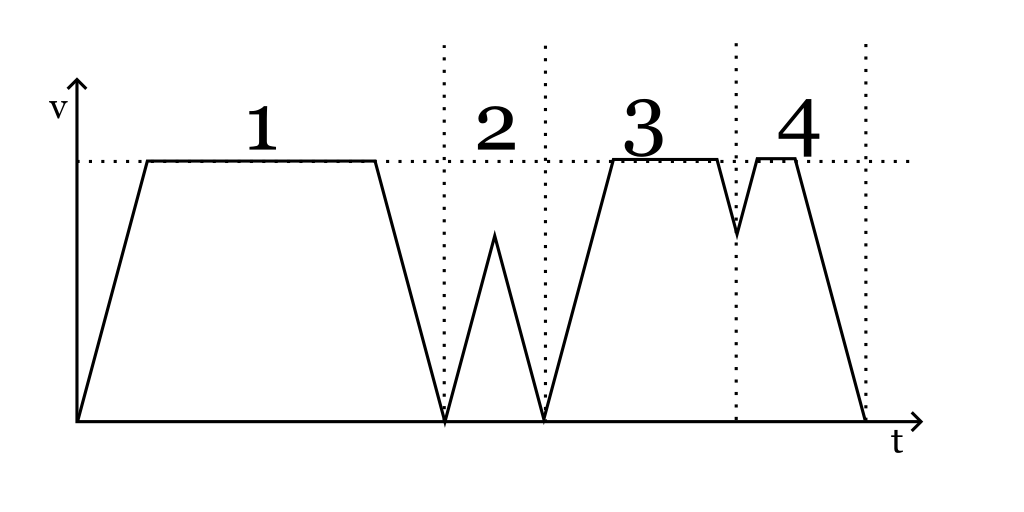
\includegraphics[scale=0.5]{trap_triang}
    \label{fig:trap_triang}
\end{figure}


\subsection{Técnicas de Controle}

\subsection{\textit{Feedforward}}
Nos métodos de controle para impressoras 3D \textit{Fused Deposition Modeling} (FDM), o controle \textit{feedforward} se consolida como a estratégia mais eficaz para os eixos de movimento, especialmente quando se pondera as restrições orçamentárias típicas de impressoras 3D padrão.

O controle \textit{feedforward} é uma abordagem utilizada em sistemas automáticos, destinada a antecipar e corrigir possíveis perturbações que possam interferir em um sistema. Ele atua proativamente, antes que tais perturbações comprometam a saída prevista. Essa técnica é especialmente útil em sistemas onde é possível prever com exatidão as perturbações.

No universo das impressoras 3D, que são tipicamente menos susceptíveis a interferências externas, é factível prever o comportamento dinâmico da máquina com precisão, baseando-se em um modelo apropriado, e sem a necessidade de sensores de alto custo. Assim, o controle \textit{feedforward} emerge como uma solução prática para otimizar o desempenho de impressoras já em operação, exigindo alterações físicas mínimas e simples ajustes no \textit{software}.

Contudo, a implementação do controle \textit{feedforward} em impressoras 3D apresenta desafios. Entre eles, a complexidade em estabelecer um modelo fidedigno, a demanda por capacidade computacional significativa e a obrigação de simular o processo de impressão do começo ao fim, considerando a influência do estado inicial \cite{ramani20,duan18}

\subsubsection{\textit{Input Shaper}}
Ao entender a trajetória pretendida e as peculiaridades do sistema, podemos deduzir uma sequência de comandos que ajustam o comando de referência com base nessas características. O objetivo é alinhar a trajetória final o máximo possível ao comando de referência. No entanto, em vez de processar todo o comando inicial, podemos adaptá-lo em tempo real usando um filtro especializado. O \textit{Input Shaper} é uma abordagem exemplar desse tipo de filtro, onde diversos \textit{Shapers} são formulados considerando variados propósitos e limitações.

O \textit{Input Shaping} é uma metodologia de controle criada para atenuar ou anular vibrações indesejadas em sistemas mecânicos ou estruturas manipuladas por atuadores, como em robôs, veículos e equipamentos industriais. Essa estratégia aprimora a sequência de pulsos de entrada, concebendo-os de modo a suprimir a ativação das frequências naturais de ressonância do sistema. Assim, o Input Shaping desempenha um papel crucial na diminuição da resposta vibratória, conferindo maior precisão e estabilidade ao sistema durante a realização de movimentos ou operações.

O valor do \textit{Input Shaping} é evidente em sistemas de controle de alta exatidão, como na robótica, onde a supressão de vibrações é fundamental para a excelência operacional e o posicionamento acurado. Utilizando o entendimento das especificidades do sistema e da trajetória almejada, essa técnica ajusta os comandos de entrada para evitar a ativação das frequências vibratórias intrínsecas, originando sistemas de controle mais robustos e eficientes. \cite{singhose97}. A Figura \ref{fig:degr_vs_esc} ilustra uma comparação entre as respostas ao estímulo de degrau e a função escalonada aplicada pelo \textit{shaper}.

\begin{figure}[H]
    \centering
    \caption{Comparação da resposta ao degrau e da resposta a escada}
    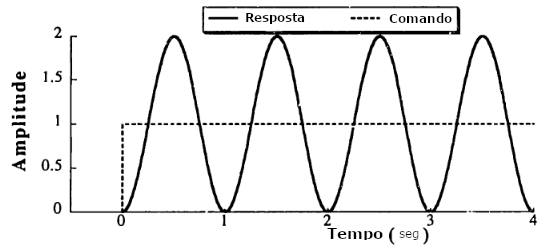
\includegraphics[scale=0.5]{inputshaperstepresponse1order}
    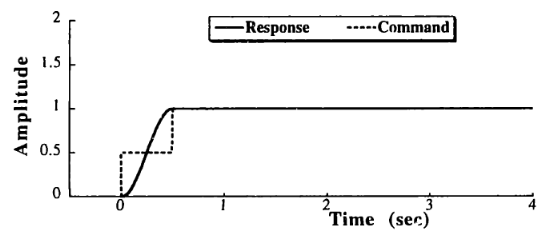
\includegraphics[scale=0.5]{inputshaperstarcasepresponse}

    {\footnotesize Fonte: \citeauthor{singhose97}, \citeyear{singhose97}}
    \label{fig:degr_vs_esc}
\end{figure}

\subsubsection{\textit{Filtered basis function (FBF)}}
O método FBF necessita que a trajetória a ser rastreada seja totalmente conhecida e que a trajetória controlada possa ser expressa como uma combinação linear de funções base possuindo coeficientes desconhecidos. As funções base são utilizadas em um controle \textit{feedforward} utilizando o modelo dinâmico do sistema e selecionando os coeficientes de maneira a minimizar os erros dada uma trajetória desejada (figura \ref{fig:flowchart_fbf}).
\cite{ramani17}

\begin{figure}[H]
    \centering
    \caption{Fluxograma FBF}
    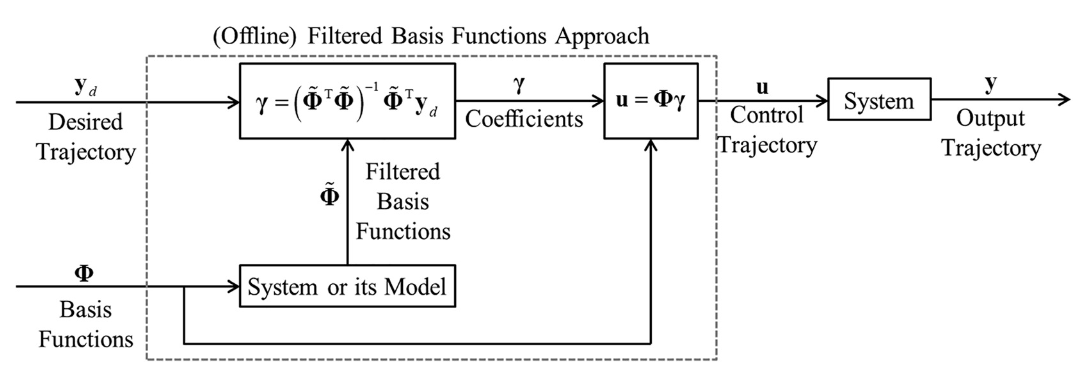
\includegraphics[scale=0.5]{ramani17blockfbf}

    {\footnotesize Fonte: \citeauthor{ramani17}, \citeyear{ramani17}}
    \label{fig:flowchart_fbf}
\end{figure}

Uma das maiores dificuldades que os métodos avançados para o controle \textit{feedforward} de trajetórias é a necessidade de se conhecer completamente a trajetória desejada, o que implica em um grande custo computacional, principalmente em situações onde são necessárias uma grande quantidade de amostras da trajetória, por exemplo em casos de alta resolução e casos de longa duração. O \textit{limited-preview filtered B-splines} adapta a solução do FBF de forma a dividir a trajetória desejada em subgrupos com um número menor de amostras e utiliza um algoritmo de \textit{receiding horizon} para calcular recursivamente os coeficientes da função B-spline que minimizam os erros de trajetória \cite{duan18}.

A partir dessa otimização da divisão da trajetória em subgrupos, esse método conseguiu ser testado utilizando uma impressora 3D de verdade com modelos simples.

Com base nos desenvolvimentos nos trabalhos de \cite{ramani17} e \cite{duan18}, comentados anteriormente, \cite{ramani20} busca atacar um segundo desafio pratico na implementação da FBF, sendo o primeiro desafio prático o custo computacional que foi endereçado pelo trabalho de \cite{duan18} através da LBFBF, permitindo a aplicação do algoritmo no mundo real.

Este segundo desafio se trata da degradação de precisão de rastreamento da abordagem FBF, causada por imprecisões no modelo ou incertezas na dinâmica da planta atrelado a característica do método de se utilizar puramente uma abordagem de \textit{feedforward}. A não participação de \textit{feedbacks} sensoriais do mundo real abre espaço para uma crescente divergência entre o modelo e a realidade.

Considerando o requisito de manter a performance computacional alcançada com o método LPFBF, \cite{ramani20} propõe, também, a utilização de um filtro robusto em substituição à dinâmica nominal da planta para filtrar as funções de base. Esse filtro robusto é construído com base no inverso de um controlador \textit{feedforward}ótimo, que minimiza uma função de custo de erro para lidar com a incerteza conhecida da planta como um filtro robusto. O esquema do método é apresentado na figura \ref{fig:flowchart_rfbf}.

\begin{figure}[H]
    \centering
    \caption{Fluxograma RFBF}
    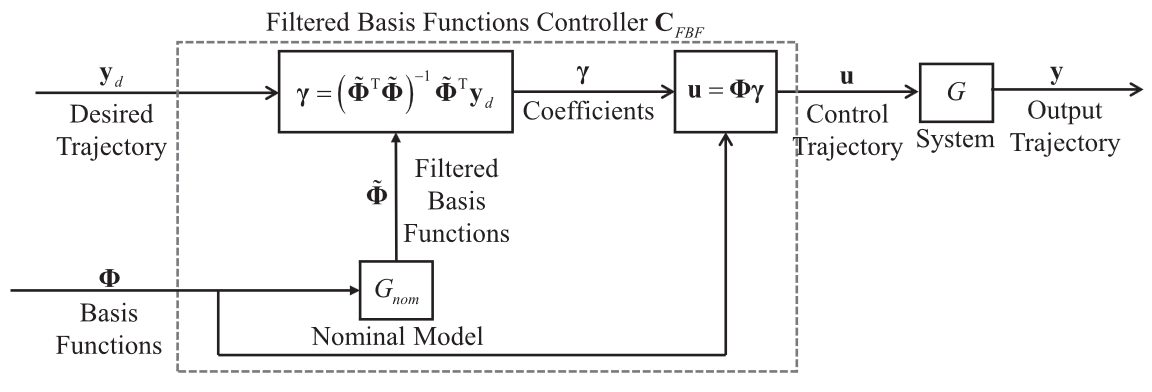
\includegraphics[scale=0.5]{ramani20blockfbf}

    {\footnotesize Fonte: \citeauthor{ramani20}, \citeyear{ramani20}}
    \label{fig:flowchart_rfbf}
\end{figure}

\section{Espaço de Estados}

Os sistemas dinâmicos podem ser descritos através de uma formulação chamada de espaço de estados, que tem como objetivo expressar modelos de equações diferencias parciais (EDP) ou ordinárias (EDO) de ordem superior como um conjunto de EDPs ou EDOs de primeira ordem. Na equação \ref{eq:edo_ex} podemos observar uma EDO de segunda ordem representando um sistema massa mola simples, logo abaixo (\ref{eq:espaco_de_estados_ex}) a mesma equação representada na formulação de espaço de estados \cite{hamilton94}.

\begin{equation}
    \label{eq:edo_ex}
    m \ddot x+c \dot x+kx = f(t)
\end{equation}

\begin{equation}
    \label{eq:espaco_de_estados_ex}
    \begin{bmatrix}
        \dot x \\
        \ddot x
    \end{bmatrix}
    =
    \begin{bmatrix}
        0 & 1 \\
        k/m & c/m
    \end{bmatrix}
    \begin{bmatrix}
        x \\
        \dot x
    \end{bmatrix}
    +
    \begin{bmatrix}
        0 \\
        1
    \end{bmatrix}
    f(t)
\end{equation}

\section{Integração implícita utilizando programação não linear}

\citeauthor{hargraves87} (\citeyear{hargraves87}) descreve um algoritmo para a solução numérica direta de problemas de controle ótimo. Este algoritmo emprega uma abordagem que utiliza polinômios cúbicos para representar as variáveis de estado. Adicionalmente, recorre à interpolação linear para tratar as variáveis de controle. Esse enfoque converte efetivamente o problema de controle ótimo em um problema de programação matemática.

Uma das principais vantagens desse método é sua facilidade de implementação e sua capacidade de lidar com uma ampla gama de problemas de otimização de trajetória. Isso inclui a consideração de restrições de caminho, estados descontínuos e desigualdades de controle.

O método alcança sua aproximação das soluções das equações diferenciais através da subdivisão de cada estado na matriz de espaço de estados em segmentos. Cada um desses segmentos é representado por polinômios de terceiro grau.

Os valores de estado são então selecionados de maneira a garantir que a curva resultante da concatenação desses polinômios seja continua, ou seja, o valor da função e de sua derivada precisa ser igual para ambos polinômios nas conexões como observado na figura \ref{fig:hargraves_fun}

\begin{figure}[H]
    \centering
    \caption{Ilustração integração implícita}
    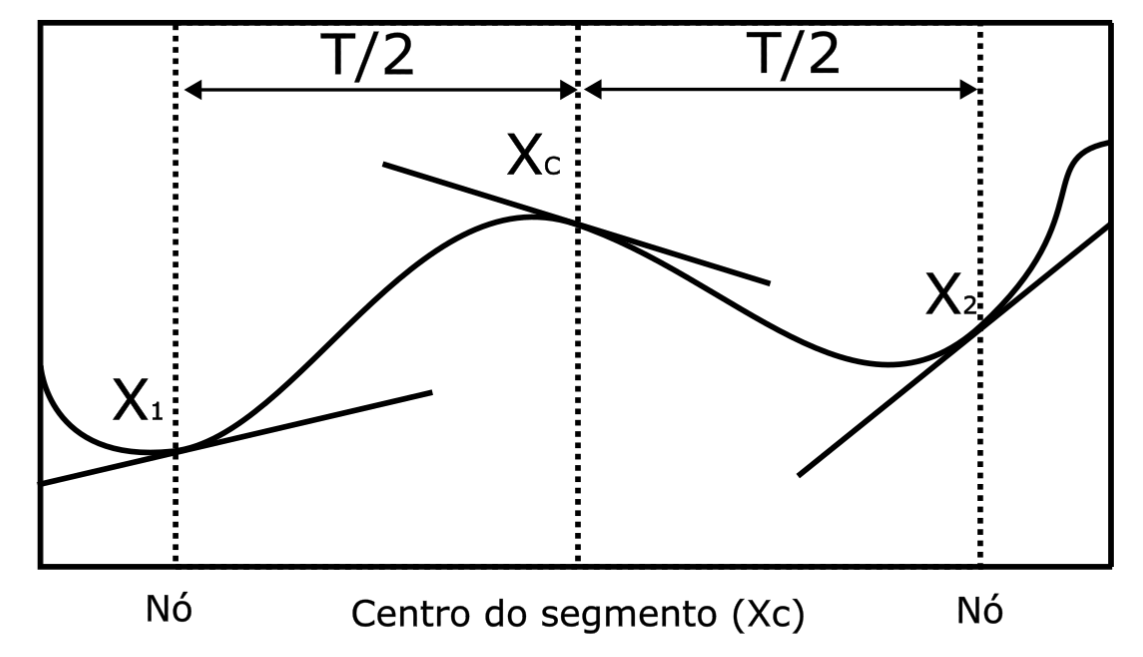
\includegraphics[scale=0.5]{hargraves_func}

    {\footnotesize Fonte: \citeauthor{hargraves87}, \citeyear{hargraves87}}
    \label{fig:hargraves_fun}
\end{figure}

O procedimento base pode ser aplicado pelos seguintes passos.

A equação \ref{eq:state_center_segment} avalia o estado no centro do segmento, onde $x$ representa o estado, T representa o comprimento do segmento e $f_i$ representa o valor da função avaliado em $x_i$. O subscrito c representa o centro do segmento.

\begin{equation}
    \label{eq:state_center_segment}
    x_c = \frac{x_{1} + x_{2}}{2} + T\frac{f_{1} - f_{2}}{8}
\end{equation}

Da mesma maneira sua derivada é apresentada na equação \ref{eq:state_dot_center_segment}.

\begin{equation}
    \label{eq:state_dot_center_segment}
    \dot{x_{c}} = -3\frac{x_{1} + x_{2}}{2T} + \frac{f_{1} + f_{2}}{4}
\end{equation}

A equação \ref{eq:defect_calc} define então o valor do defeito no centro do segmento.

\begin{equation}
    \label{eq:defect_calc}
    \Delta = f_c - \dot{x_c}
\end{equation}

Considerando também que a entrada do sistema pode ser avaliada de forma aproximada no centro do segmento através da equação \ref{eq:input_value_center_segment}.

\begin{equation}
    \label{eq:input_value_center_segment}
    u_c = \frac{u_1 + u_2}{2}
\end{equation}

Os valores de estado agora podem ser alterados de maneira que o defeito tenda a zero.